\chapter{Hypothesis and research questions}
\label{chp:innovative_chapter}

\graphicspath{{chapter_3/figures/}} % path to the figures folder of this chapter

\section{Knowledge gap in the current state of the art}
\label{Knowledge gap in the current state of the art}
The current use and experimentation in the field of FFF tries to bridge the gap between simple consumer parts towards functional and mechanically reliable parts. For this a significant amount of effort has been put in the characterization of mechanical properties trough loading tests, including the effect process parameters have on the samples. It has been concluded that the properties are dramatically different from bulk material due to porosity and weak bonding area's. To be able to predict the properties of these anisotropic properties, different approaches have been proposed by multiple researchers, with considerable effort from  Rodriguez et al\cite{Rodriguez2003MechanicalModeling}. 

To determine the effect of the porosity on a FFF product the mesostructure is first analysed by using microtoming. The results from different systems can significantly alter in mesostructure, the quality and accuracy of the mechatronics are most likely the cause of this deviance. Due to the different observations no clear agreement was concluded between the researchers on the formation of this porosity. The UMS5 is currently one of the most advanced FFF systems that show promising results with a reproducible quality.

The empirical loading tests conducted by different researchers often used testing standards for isostropic polymers. The geometry of the samples used resulted in stress concentrations and crack initiation points, causing the samples to fail prematurely. Additionally, the production procedure is not yet standardized, meaning that the produced samples show significant difference between research methodologies and alter in quality.

There have been several attempts to analyze and predict the degree of bonding of the road interface. Since this is a complex time dependant parameter, no exact prediction was made to this date on the bonding between roads. Most researchers assumed perfect healing (bulk properties) of the interface. 

Multiple researchers found overlap between FFF products and composites, therefore they applied elasticity models such as the mechanics of materials approach and the Classical Laminate Theory to FFF products. Additionally, a few Finite Element Analysis where performed to determine the elastic properties of FFF products. The results of the elastic models are in accordance with the experimental results.

Since the non-linear behaviour of polymers is complex and hard to predict, due to their molecular structure and strain rate dependency, the FEM knowledge on this topic is limited. For composites that incorporate an epoxy and long fibres, some validated models have been proposed on a micro-mechanical scale.  Epoxies have a more predictive non linear behaviour due to their cross-links. If the understanding of polymer molecular behaviour is sufficient, one could try to adjust the composite model to simulate the micro mechanical properties of FFF products. 

%The issue is that different FFF systems exhibit significant difference in produced quality.
\section{Hypothesis}
Based upon the knowledge gap defined in previous section the following hypothesis has been formulated.

"FFF products show large anisotropy due to a limited degree of bonding between roads and significant amount of porosity. The porosity could be analyzed with mircrographs before implementing a composite RVE model to determine the elastic and non-linear properties of FFF products. These result could be validated with empirical loading tests."

%"The characteristics involving the degree of bonding and the porosity are the main contributors to the decrease of mechanical properties with respect to the bulk material, these characteristics are strongly influenced by the process parameters and hardware used. By characterizing these properties for a particular combination of material, hardware and software, models could be made that makes a valid prediction of the mechanical properties of produced parts."

\section{Research questions}
    \label{Research questions}
In order to verify this hypothesis a number of research questions has been formulated. These research questions are formulated as follow:

"What are the process parameters influencing the main characteristics,?"

"What are the optimal process parameters for the Ultimaker S5 system and what are the related mechanical properties?"

"Is there a clear geometry for the mesotructure of these FFF products, and can the formation of this structure be derived?"

"What is the optimal test and production procedure for the testing of FFF samples, and what are the related mechanical properties of the FFF samples and filament?

"Can the elastic and non-linear properties be predicted with a composite RVE micro-mechanical mode and how do this relate to other composite models?"

%"What is the influence of the negative airgap on the porosity?"

%"What is the minimum amount of porosity that is obtainable, without significantly distorting and overdimensioning the product?"

%"What model would give most realistic results predicting the mechanical properties (considering the influence of degree of bonding and porosity)?"

%"Can this model be implemented to predict the properties of complex parts with different layer orientations, different infill, material, process parameters and systems?".

%"How does this model compare to the models from literature and Digimat?

\section{Research methodology}
To answer the research questions stated in the previous section a research methodology needs to be defined. This section will describe the steps necessary to answer the research questions. 

First the literature should be studied to identify the process parameters that are influencing the mechanical properties. Additionally, it should be investigated if these parameters comply with the optimal parameters of the UMS5.

Subsequently, the mesostructure should be analyzed with micrographs to identify the form and amount of porosity in the UMS5 products.  A derivation should be searched to construct the mesostructure and consequently define the RVE, which is ideally dependant of the process parameters. 

Consequently, different empirical tests should be conducted with these parameters for the UMS5. The different test procedures should be compared with each other to determine the optimal testing method that will result in most representative response for the bulk product. Also, filament should be tested to determine the bulk properties of the material.

Furthermore, the RVE defined from the mesostructure can be used with the elasticity and non-linear composite models. First these models need to be adjusted to the FFF characteristics. Important here is to get a good understanding of the mechanical behaviour of thermoplastic polymers, and implement the correct constitutive equations in the RVE model. Besides the RVE model, other analytical models can be compared to determine it's effectiveness.  

Finally, it is important to validate the adjusted RVE model to the empirical tests and verify it with the other analytical models. The RVE model can afterwards be validated for different process parameters when additional process parameters are empirically tested. 


%The research methodology is based on the enhancement model that is based on a composite RVE model. To obtain data that can be implemented in the model and data that is needed to verify and validate the model and create iterations, empirical tests are done alongside the development of the model. 

\begin{figure}[H]
    \centering
    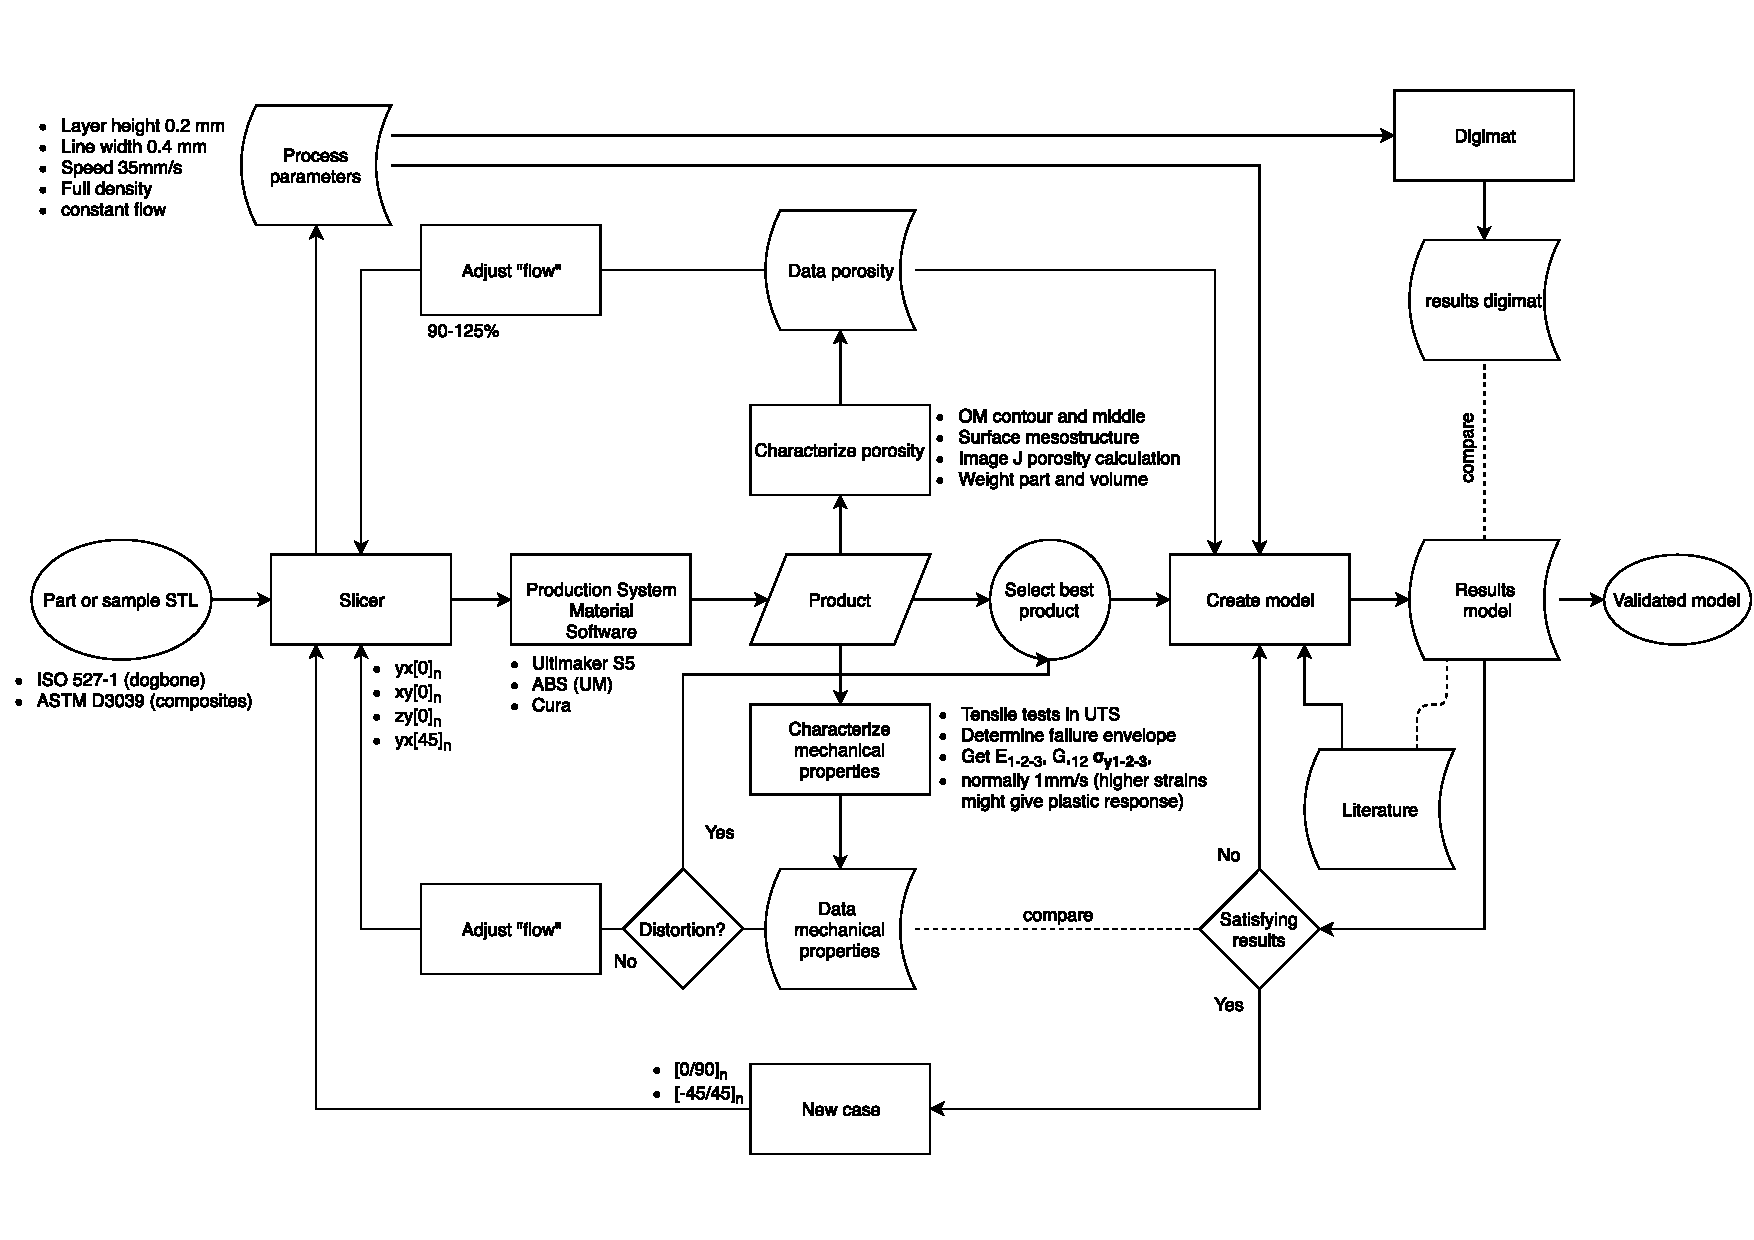
\includegraphics[width=1\textwidth]{chapter_3hypothesis/figures/Testmethod2.pdf}
    \caption{Test methodology}
    \label{fig:Test methodology}
\end{figure}

%The research mehtodology is based on the research questions stated in section \ref{Research questions}, the methodology presented aims to define the steps necessary to answer the research questions and subsequently verify or reject the proposed hypothesis. 
%First the results of the Ultimaker S5 systems should be analyzed to compare them with the results of the literature, and determine if the focus of the model should be configured. This includes an analysis on the porosity and mechanical properties. If time allows, an analysis on the thermal history should also be done to get a better view on the degree of bonding of the layers.
%Subsequently, the best parameters should be defined for producing FFF parts with the Ultimaker S5. The effect of most parameters are known, except for the increase in flow of the parts to decrease the prososity of the part. Literature has proven that it can significantly reduce the porosity for other systems, it would be important to know if this would also stand for the Ultimaker S5 system.
%Simultaneously, the dimension of the part should be examined to determine if no unacceptable distortion takes place due to overextrustion.
%When the best parameters are defined, the information generated on the porosity can be used to enhance the model, the model can then be verified and validated according to the mechanical properties. The implementation of cohesive elements/zones might be needed to simulate the best results.
%Furthermore, the model can be used to simulate different scenarios, e.g. $yx[-45/45]_n$, to validate the different cases mechanical testing should be done.
%Additionally, the software used in Digimat should be compared to the findings from the produced model. The software in Digimat applies a plasticity model that could also be introduced in the produced model, however, the benefits from this might be insignificant due to the small plastic response from FFF produced parts. Better would be to generate an additional strength model to determine the UTS and yield strength.
%Finally, the models from the literature, Digimat and mechanical experiments should be compared to the produced model to validate and verify it. Additionally, different cases could be investigated to analyze if these also hold for the model.




